\subsubsection{Minuta de reunião (11-Junho-2015)}

\begin{tabbing}
  Local \= xxx \kill
  Local \> : LEAD \\
  Data  \> : 11 de Junho de 2015 \\
  Hora  \> : 9:00
\end{tabbing}

%---------------------------------------------------------------------
\participantes{
  \elael,
  \alana,
  \gabriel,
  \julia,
  \ramon,
  \renan.
}

\textbf{Aprovação da minuta}

\textbf{Update semanal do Projeto EMMA}
   
\textbf{\julia.} 
	\begin{itemize}
		\item \textbf{Tarefas concluídas:}
			\begin{itemize}    
				\item Apresentação EMMA.
				\item ADM/ Documentos /Viagem
			\end{itemize}
		
		\item \textbf{Novas tarefas:}
			\begin{itemize} 
				\item Atualizar documentação.
				\item Finalizar apresentação.
				\item Mestrado: questões relaciondas ao tema de controle de missão
				robótica.
			\end{itemize}
	\end{itemize}
					
		
\textbf{\elael.} 
	\begin{itemize}
		\item \textbf{Tarefas concluídas:}
			\begin{itemize}    
				\item Checou menor velocidade que possível para a base que permite a
				aplicação continua de coating.
				\item \item Calculou valores de torc.
			\end{itemize}
		
		\item \textbf{Novas tarefas:}
			\begin{itemize} 
				\item Formalizar ajustes no EMMA SOTA.
				\item Estudo sobre Shutter.
				\item Auxiliar estevão no desenho da Base.
			\end{itemize}
	\end{itemize}
					
\textbf{\gabriel.} 
	\begin{itemize}
		\item \textbf{Tarefas concluídas:}
			\begin{itemize}    
				\item analisouparafusos magnéticos.
				\item Modelo 3D em OpenRave.
			\end{itemize}
		
		\item \textbf{Novas tarefas:}
			\begin{itemize} 
				\item Formalizar ajustes no EMMA SOTA.
				\item Checar viabilidade de operaçào no espaço atrás das pás.
				\item Verificar manipuladores.
			\end{itemize}
	\end{itemize}
					
			
   \textbf{\estevão.} 
	\begin{itemize}
		\item \textbf{Tarefas concluídas:}
			\begin{itemize}    
				\item Trabalhou no modelo 3D da unidade geradora.
			\end{itemize}
		
		\item \textbf{Novas tarefas:}
			\begin{itemize} 
			    \item Terminar modelo 3D da unidade geradora.
				\item Desenho da base com Elael.
			\end{itemize}
	\end{itemize}

			



\textbf{Agenda para a próxima reunião:}
  \begin{itemize}
    \item Resultado de pesquisas individuais.
    \item Novas tarefas \& recomendações.
  \end{itemize}


\vspace{5mm}%
\parbox[t]{70mm}{
  Aprovado por: \\[5mm]
  \centering
  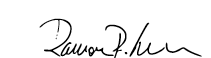
\includegraphics[width=65mm]{figs/logo/assinatura-ramon.png} \\[-4mm]
  \rule[2mm]{70mm}{0.1mm} \\
  \ramon \\[1mm]
  Coordenador do Projeto \\
}

%---------------------------------------------------------------------
\fim